\documentclass[9pt,twocolumn,twoside]{../../styles/osajnl}
\usepackage{fancyvrb}
\journal{i524} 

\title{HTCondor: Distributed Workflow Management System}

\author[1,*]{Niteesh Kumar Akurati}

\affil[1]{School of Informatics and Computing, Bloomington, IN 47408, U.S.A.}

\affil[*]{Corresponding authors: akuratin@indiana.edu}

\dates{paper1, \today}

\ociscodes{HTCondor, ClassAd, Match Making, Condor-G, High-throughput Computing, Cycle Scavenging, Batch Systems}

% replace this with your url in github/gitlab
\doi{\url{https://github.com/Niteesh01/sp17-i524/blob/master/paper1/S17-IR-2001/report.pdf}}


\begin{abstract}
HTcondor is a distributed high throughput computing open-source
workflow management system developed by the condor research team at
University of Wisconsin-Madison Department of Computer Sciences. It is
an unique and highly sophisticated Job Scheduler which has been
changing and adopting dynamically in alignment with the users and the
growing popularity of the distributed computing field. It is used for
distributed parallelization of computing intensive tasks. The Condor
project has become popular for its two key products, they are: The
Condor high-throughput computing system, and the Condor-G agent for
grid computing.\newline
\end{abstract}

\setboolean{displaycopyright}{true}

\begin{document}

\maketitle

% Condor

\section{Introduction}
An ideal computing environment provides ready access to huge scale of
computing power. Over the course of years it is recognized that such
immense computing power can be achieved at a very low cost by
combining various small devices rather than using expensive
supercomputers. This situation is addressed by the condor project.
The core philosophy of the Condor project is flexibility.

``Like other full-featured batch systems, HTCondor provides a job
queueing mechanism, scheduling policy, priority scheme, resource
monitoring, and resource management. Users submit their serial or
parallel jobs to HTCondor, HTCondor places them into a queue, chooses
when and where to run the jobs based upon a policy, carefully monitors
their progress, and ultimately informs the user upon
completion''\cite{beowulfbook-condor} Apart from providing the
functionalities as other batch systems, HTCondor harnesses effectively
wasted CPU cycles from idle desktops as well as workstations by using
various effective mechanisms.

HTCondor is really unique because it can be used for managing workload
on a set of dedicated clusters like the beowulf clusters, thereby
allocating work to idle desktops/workstations the process being called
as cycle scavenging. ``HTCondor can seamlessly integrate both
dedicated resources (rack-mounted clusters) and non-dedicated desktop
machines (cycle scavenging) into one computing
environment''\cite{HTCondor_wikipedia}

\section{Architecture}

At the core of HTCondor technology lies the kernel.The kernel shown in
Fig.1 is the fundamental structure of HTCondor. Computing environments
with wide variety can be constructed by making minor modifications to
the kernel. The kernel workflow is as follows a user submits a job to
an agent, the agent remembers the job in a persistent storage while
looking for resources that are willing to run the job. Matchmaker is
responsible for potential agents and resources. The agents and
resources advertises themselves to the matchmaker. The matchmaker
introduces the agent, the agent once introduced is responsible for
contacting the resource and validating the match.To execute a job both
agent and resource starts new processes called shadow and sandbox
respectively. Shadow provides all the details necessary to execute a
job. Sandbox creates a safe environment to run the job
\cite{condor-practice}


%\subsection{Sample Figure}

%Figure \ref{fig:The Condor Kernel}.

\begin{figure}[htbp]
\centering
\fbox{\includegraphics[width=\linewidth]{images/Condor_Kernel.eps}}
\caption{The HTCondor Kernel}
\label{fig:condor-practice}
\end{figure}

\section{The HTCondor Software}
HTCondor project supports a variety of computing systems deployed
worldwide for various commercial and academic purposed. The HTCondor
products: The Condor high-throughput computing system, and the
Condor-G agent for grid computing are very popular among various
domains. Lets discuss both these products in detail


\subsection{HTCondor High Throughput Computing System}
HTCondor being a high-throughput distributed batch computing system.
It provides job management, scheduling, resource management and
monitoring just like other batch systems. HTCondor is prominent in
areas where other batch systems are weak like:high-throughput
computing, and oppurtunistic computing. The idea of high-throughput
computing is providing large amounts of computing power that is fault
tolerant over prolonged periods of time by effectively utilizing the
resources that are available in the network. Oppurtunistic computing
is to use resources whenever they are available. High-throughput
computing can be efficiently achieved through oppurtunistic
computing. Therefore, HTCondor brings together high-throughput
computing as well as oppurtunistic computing

%\begin{description}
To achieve high-throughput computing through oppurtunistic means, this
requires several powerful as well as unique tools:

\begin{itemize}
%\renewcommand{\labelitemi}{\scriptsize$\square$} 

\item {\bf ClassAds.} ``The ClassAd language in Condor provides an
  extremely flexible and expressive framework for matching resource
  requests(e.g jobs) with resource offers (e.g
  machines)''\cite{condor-practice}.  The ClassAd mechanism makes it
  easy for the job to state the requirements and preferences of the
  job. It also makes it easy for the machines to specify about the
  preferences and requirements for the jobs they are willing to run.
  Therefore, enabling these resources and requirements to be described
  in the form of powerful expressions thus resulting in HTCondor's
  adoption mostly any desired policy\cite{condor-practice}
  
\item {\bf Job Checkpoint and Migration.} A Job checkpoint is a
  snapshot of the complete state of the
  job\cite{Checkpoint_Migration_techreport_1997}. With certain types
  of jobs HTCondor can take a checkpoint of the job and later resume
  it. Job can continue its execution later exactly from it left off at
  the time of checkpointing. HTCondor also allows job migration from
  one pool of resources to an other pool of resources with the help of
  checkpointing\cite{beowulfbook-condor}

\item {\bf Remote System Calls.} HTCondor preserves the local
  execution enviroment using remote system calls despite running jobs
  on remote machines. Users need not make files available on remote
  workstations by accessing the machines using remote login. Remote
  system calls is a mobile sandbox mechanism of HTCondor which is used
  for redirecting all the I/O related calls back to the machine which
  submitted the job. The program behaves as if it is running on the
  originally submitted workstation, regardless of where it really
  executes\cite{condor-practice}
  
\end{itemize}
%\end{description}\cite{condor-practice}

HTCondor with the help of above tools can also scavenge and manage
wasted CPU power from otherwise idle workstations across the
organization with minimal effort\cite{condor-hunter}. The same
mechanisms enable preemptive-resume scheduling on compute cluster
resources. Therefore, this allows HTCondor to support priority based
scheduling on clusteres. HTCondor therefore can be used to combine all
of organization's computing power into a single resource.

\subsection{Condor-G}

The Condor-G is combination of initiatives from Globus and HTCondor
projects. Globus is about inter-domain communications as well as
standardized access to a variety of remote batch
systems\cite{Globus1997article}. In HTCondor comes the user concerns
of fault tolerance, error recovery, creating a friendly execution
environment, job submission and job allocation

``Condor-G can be used as the reliable submission and job management
service for one or more sites, HTCondor can exist both at front end
and back end of a grid. The HTCondor HTC system can be as the fabric
management service for one or more sites and the Globus Toolkit can be
used as the bridge between them''\cite{condor-practice}.

\section{ClassAd Mechanism}
The ClassAd mechanism is an unique, extremely flexible mechanism for
handling jobs and resource requests. HTCondor uses matchmaking for
matching an idle job with an available machine. ClassAds are used by
users to specify which machines should service their
jobs. Adminstrators uses it customize the sccheduling policy.

HTCondor's ClassAd mechanism is similar to the classifieds in the
advertising section of the newspaper. Sellers advertise what they hope
to sell to attract the buyers at the same time buyers advertise
specifics whar they wish to purchase.

ClassAds consists of a unique set of named expressions. Each
expression is an attribute. Each attribute has an attribute name as
well as value\cite{ClassAddstechreport2003}.

\section{DAGMan}
DAGMan is a problem solver which is a higher-level structure built on
top of the HTCondor agent. It provides an unique programming model for
managing large number of jobs. A problem solver relies/uses agent as a
service for reliable execution of jobs. Therefore, the problem need
not worry about failure of jobs as the agent assumes responsibility
for hiding and retrying those jobs.

DAG Manager(DAGMan) is a service responsible for execution of multiple
jobs with dependencies in a declarative form. DAGMan is a fault
tolerant as well as distribute version of traditional tool make.  DAG
does not depend on the file system to record a DAG process unlike
make.  DAG keeps a set of private logs to act in the case of crashes
or failures



\section{Applications}
HTCondor has been adopted widely across various commercial and
academia. Few of the notable applications in academia and commercial
space are listed here: C.O.R.E Digital Pictures, NUG30 Optimization
Challenge


\begin{itemize}

\item{\bf C.O.R.E DIgital Pictures.} A highly successful Toronto-based
  computer animation studio. The studio primarily deals primarily with
  Photo-realisitic animation which is a compute intensive process.
  Each frame can take upto 1 hour. An animation requires 30 or more
  such frames. Today, HTCondor manages hundreds of linux and silicon
  Graphics machines at C.O.R.E Digital Pictures. On a average day
  15000 jobs are submitted by the C.O.R.E animators to
  HTCondor. HTCondor has been successfully used by C.O.R.E for major
  productions such as X-Men, Blade II nd The Time Machine

\item{\bf NUG30 Optimization Challenge.} NUG30 is quadratic assignment
  problem first proposed in 1968 as one of the most difficult
  combinatorial optimization challenges, but remained unsolved for 32
  years beacuse of its complexity. This problem is solved by four
  mathematicians from Argone National Laboratory, University of Iowa,
  and Northwestern University by using Condor-G and several other
  technologies

  The actual computation was managed by HTCondor's Master-Worker(MW)
  problem solver environment.'' MW submitted work to Condor-G, which
  provided compute resources from around the world by both direct
  flocking to other Condor pools and by gliding in to other compute
  resources accessible via the Globus GRAM protocol. Remote System
  Calls, part ofCondor’s standard universe, was used as the I/O
  service between the master and the workers. Checkpointing was
  performed every 15 minutes for fault
  tolerance''\cite{condor-practice}

 As a result a solution to NUG30 was discovered by utilizing Condor-G
 in a run of less than one week. Condor-G allowed the mathematicians
 to manage 2400 systems at 10 different sites seamlessly. Over 95,000
 CPU hours are consumed in that week\cite{condor-practice}
 
\end{itemize}

\section{Educational Material}

HTCondor is one of the most popular technology for high-computing
distributed workflow management system. More information about
HTCondor can be found here \cite{HTCondor_website}.

\section{Licensing}

HTCondor is released under the open source Apache License, Version
2.0. You may not use this file except in compliance with the
License. You may obtain a copy of the License
here\cite{HTCondor-License}.

\section{Conclusion}

HTCondor is a powerful, unique and flexible high throughput computing
distributed workflow management system which has evolved over years by
keeping the end users,adminstrators and the growing demand in
mind. HTCondor continues to standout from other batch management
systems with the power of high-throughput computing and oppurtunistic
computing.

%Condor



% Bibliography

\bibliography{references}

\newpage

\appendix




\end{document}
